\documentclass[11pt,a4paper]{article}

\usepackage[margin=1in]{geometry}
\usepackage{amsmath,amssymb}
\usepackage{booktabs}
\usepackage{tabularx}
\usepackage{array}
\usepackage{graphicx}
\usepackage{float}
\usepackage{xcolor}
\usepackage{hyperref}
\usepackage{enumitem}
\usepackage{tikz}
\usetikzlibrary{arrows.meta,positioning,shapes.geometric}

\hypersetup{
    colorlinks=true,
    linkcolor=black,
    citecolor=blue!60!black,
    urlcolor=blue!60!black
}

\setlist[itemize]{leftmargin=*, topsep=3pt, itemsep=2pt}
\setlist[enumerate]{leftmargin=*, topsep=3pt, itemsep=2pt}
\renewcommand{\arraystretch}{1.15}

\newcommand{\pcu}{PCU}
\newcommand{\od}{O--D}
\newcommand{\figurepanel}[2]{%
\IfFileExists{#1}{%
  \includegraphics[width=\linewidth]{#1}%
}{%
  \fbox{%
    \begin{minipage}[c][0.28\textheight][c]{0.94\linewidth}
      \centering
      \textbf{Figure}\\[4pt]
      #2\\[4pt]
      Source file: \texttt{\detokenize{#1}}.
    \end{minipage}
  }%
}%
}

\title{\textbf{Methodology Documentation}\\
\large Nepal National-Highway Input Network and Origin--Destination Estimation}
\author{Prepared for methodology documentation}
\date{Latest update: 10 July 2026}

\begin{document}
\maketitle

\begin{abstract}
This document brings together the preparation of the project's national-highway
input and the existing origin--destination estimation methodology. The master
highway layer, \texttt{Nepal.gpkg}, layer \texttt{NH}, contains 718 link-level national-highway
features with cleaned identifiers, topology repairs, design speeds and two
AADT fields. The modelled mean speed is derived from design speed during graph
construction. The same GeoPackage also carries the
supporting context layers needed for later modelling: district-headquarter
areas, country boundary, health facilities, airports and settlement points. The OD calibration is
now intended to use the \texttt{AADT\_2023} field from this master input, because
the 2023-side SSRN coverage is much more complete than the 2024/25 station
sample. The second part documents the gravity seed matrix and entropy-based
ME2/ODME procedure used to estimate inter-district demand. Keeping the two
parts together makes it clear which quantities are observed, which are
modelled, and how the road inputs support the later OD workflow.
\end{abstract}

\part{National-Highway Input Network}

\section{Purpose and Final Deliverable}

\texttt{Nepal.gpkg} is the project's master spatial input. Its highway layer,
\texttt{NH}, is in WGS 84 (EPSG:4326) and contains 718 LineString
national-highway features. A feature represents an official highway link,
rather than a short routing edge. This explains why the layer contains far
fewer features than the OSM-derived graph: the difference is segmentation, not
necessarily network coverage.

The file also includes contextual layers that support OD and accessibility
work, including district-headquarter areas, health facilities, airports,
settlements and the country boundary.

\section{Source Preparation and Attribute Cleaning}

The source was a GeoRSS response from the national-highway GeoServer layer. Its
attributes were embedded as HTML inside a single \texttt{description} field.
Those values were parsed into normal fields, including
\texttt{road\_refno}, \texttt{link\_code}, \texttt{link\_name},
\texttt{link\_from}, \texttt{link\_to}, terrain and road class.

\texttt{link\_code} is the unique link identifier, for example
\texttt{NH07-004}. The shorter \texttt{road\_refno}, such as \texttt{NH07}, is
retained because it provides the highway grouping needed for summaries and
nearest-link imputation. The two fields therefore serve different purposes and
should not be treated as duplicates.

The official link length is retained as \texttt{link\_len}, rounded to two
decimal places in kilometres. It normally follows the administrative chainage
relationship

\begin{equation}
L_i^{\mathrm{chain}} = \texttt{link\_to}_i -
\texttt{link\_from}_i.
\label{eq:linklength}
\end{equation}

The source \texttt{link\_len} was retained rather than overwritten by this
calculation. All but one link agree with the chainage difference within
0.01 km; the single larger difference is 0.15 km and remains visible for later
source-data review.

\section{Topology Audit and Repair}

An endpoint-only screening initially identified 255 apparent dangling
endpoints. A more complete audit showed that 179 already coincided with an
internal vertex of another highway link and were therefore connected. Of the
remaining cases, 20 endpoints touched another link but required an explicit
vertex on the receiving line, while four genuine gaps of no more than 1 metre
required both endpoint movement and vertex insertion. These 24 locations were
repaired.

Fifty-two endpoints were retained as network termini because joining them would
have exceeded the 1 metre rule; the nearest alternatives ranged from 1.305 m to
62.695 km away. Automatically connecting all of them would have introduced
false roads. Their separate audit point layer is not included in
\texttt{Input\_NH.gpkg}.

\begin{figure}[H]
\centering
\includegraphics[width=\linewidth]{Methodology_assets/topology_repairs_1m.png}
\caption{Locations where explicit topology repairs were applied. The map is a
documentation audit; the repair points are not separate layers in the final
input GeoPackage.}
\label{fig:topologyrepairs}
\end{figure}

\begin{figure}[H]
\centering
\includegraphics[width=\linewidth]{Methodology_assets/remaining_dangles.png}
\caption{Retained highway termini after applying the 1 metre topology rule.
These points include legitimate route ends and locations where automatic
connection would be unsafe.}
\label{fig:remainingdangles}
\end{figure}

\section{Design-Speed and Mean-Speed Assignment}

Design speed is carried by the master highway layer and follows the Nepal Road
Standard 2070 road-class speed framework \cite{dor2013}. For impedance, it is converted to a
network-wide mean operating speed using
\texttt{mean\_speed\_kmh = 0.40 * design\_speed\_kmh}.

\begin{table}[H]
\centering
\caption{Design speeds used in \texttt{Nepal.gpkg}, layer \texttt{NH}, km/h.}
\begin{tabular}{lrrrr}
\toprule
\textbf{Road class} & \textbf{Plain} & \textbf{Rolling} &
\textbf{Mountainous} & \textbf{Steep} \\
\midrule
Class I   & 120 & 100 & 80 & 60 \\
Class II  & 100 & 80  & 60 & 40 \\
Class III & 80  & 60  & 40 & 30 \\
Class IV  & 60  & 40  & 30 & 20 \\
\bottomrule
\end{tabular}
\end{table}

These are design speeds, not observed operating speeds. Design speed $V_d$
represents the geometric standard used to lay out a road. Network impedance,
however, must represent the average movement of mixed traffic under posted
speed controls, settlement influence, roadside activity, and local safety
conditions. For this reason, the model converts design speed to average
operating speed through a single empirical ratio.

Recent Nepal highway evidence supports a substantial reduction from design
speed to operating or posted speed. Bist and Tiwari \cite{bist2024} study the
NH58 Karnali Highway section at Airport Chowk--Mangalgadhi Chowk in
Birendranagar, where a section with 100 km/h design speed has 20--40 km/h
posted speeds and observed mixed-traffic speeds around 30--40 km/h. The
Butwal--Gorusinghe detailed design on the East--West Highway reports 120 km/h
design speed for NH01-046 to NH01-050, while posted controls vary across
operating contexts, including 60 km/h urban sections, 80 km/h rural sections,
and 30 km/h service roads \cite{dor2023}. In Kathmandu, the Ring Road and Outer
Ring Road are designed at 120 km/h in the improvement-project design context,
while major-road speed control is reported at 50 km/h, giving a posted-to-design
ratio of about 0.42 \cite{jica2022,ktmtraffic2023}.

\begin{table}[H]
\centering
\caption{Nepal benchmark evidence for converting design speed to operating speed.}
\small
\begin{tabularx}{\linewidth}{lrrl}
\toprule
\textbf{Benchmark section} & \textbf{$V_d$} & \textbf{Posted/observed speed} &
\textbf{Implication} \\
\midrule
NH58-007, Karnali Highway & 100 & 20--40 &
Urban highway controls and observations fall near or below 0.40$V_d$. \\
NH01-046--050, Butwal--Gorusinghe & 120 & 30--80 &
Operating controls vary by urban, rural and service-road context. \\
NH38/NH39, Kathmandu Ring Road system & 120 & 50 &
Posted/design ratio is approximately 0.42. \\
\bottomrule
\end{tabularx}
\end{table}

Based on these benchmarks, the impedance model adopts a conservative national
planning average:

\begin{equation}
V_{\text{avg},i}=0.40\,V_{d,i}.
\label{eq:mean-speed}
\end{equation}

This factor is not a posted speed limit for every individual link. It is a
network-wide mean operating-speed assumption used to convert design-speed
attributes into travel-time impedance for OD routing and MLPI scoring. The
active code writes this as
\texttt{mean\_speed\_kmh = 0.40 * design\_speed\_kmh}.

\section{AADT Fields and Matching}

The master highway layer carries two daily traffic fields in vehicles/day:
\texttt{AADT\_2023} and \texttt{AADT\_2024\_25}. The OD calibration uses
\texttt{AADT\_2023} because it provides complete link-level coverage for the
current national-highway graph. The \texttt{AADT\_2024\_25} field is retained
for comparison and future sensitivity testing.

AADT targets are matched to graph fragments by the official
\texttt{link\_code}. During graph construction, each official highway link is
split into directed fragments at intersections and HQ connector locations. The
source \texttt{link\_code} is preserved on every derived fragment, so a traffic
target for link $a$ constrains the set of graph fragments carrying the same
code. Traffic values are treated as two-way section counts because no
directional AADT split is supplied.

\begin{table}[H]
\centering
\caption{Final AADT fields in \texttt{Nepal.gpkg}, layer \texttt{NH}.}
\begin{tabular}{lrp{0.56\linewidth}}
\toprule
\textbf{Field} & \textbf{Populated links} & \textbf{Meaning} \\
\midrule
\texttt{AADT\_2024\_25} & 718 & Extrapolated to the full network using the
170 observed 2024/25 station values as the calibration base. \\
\texttt{AADT\_2023} & 718 & Mostly direct from \texttt{ssrn\_traffic.xml};
23 missing links were filled from the nearest valued link on the same highway.
This is the preferred OD calibration evidence
because its network coverage is much higher. \\
\bottomrule
\end{tabular}
\end{table}

The modelling layer therefore exposes the two traffic-year columns needed for
the current OD and MLPI workflow.

\section{Context Layers Added to the Master GeoPackage}

The same GeoPackage now includes supporting layers that will be useful for OD,
accessibility and map production:

\begin{table}[H]
\centering
\caption{Additional layers currently included in \texttt{Nepal.gpkg}.}
\begin{tabularx}{\linewidth}{p{0.24\linewidth} rp{0.48\linewidth}}
\toprule
\textbf{Layer} & \textbf{Features} & \textbf{Notes} \\
\midrule
\texttt{district\_hq} & 77 & District-headquarter areas. The source polygon
file had 154 features, two per headquarters; these paired geometries were
dissolved to 77 area features and attributed from the GeoRSS description
fields. \\
\texttt{country\_boundary} & 5,720 & Country boundary linework copied from the
project GeoPackage and reprojected to EPSG:4326. \\
\texttt{health\_facilities} & 4,091 & Point layer from the NepalBaseMap health
GeoRSS export, with description attributes converted to columns. \\
\texttt{airport} & 45 & Airport point layer from the NepalBaseMap airport
GeoRSS export, with description attributes converted to columns. \\
\texttt{settlement} & 76,264 & Settlement point layer added from the prepared
project GeoPackage. It supports accessibility and map context in the current
workflow. \\
\bottomrule
\end{tabularx}
\end{table}

\section{Final Highway-Layer Fields}

The final layer retains route and link identifiers, names, chainages,
administrative fields, terrain and road class, design speed, modelled mean
speed, and the two AADT columns. The \texttt{source\_url} field is placed last
so that the working attributes appear first in QGIS.

\part{Origin--Destination Matrix Estimation}

\section{Purpose and Modelling Position}

The objective was to obtain a defensible prior \od{} matrix and then improve it
with the traffic-count evidence available in the project data. The workflow is
therefore deliberately two-stage:

\begin{enumerate}
    \item synthesize a complete seed matrix using a doubly constrained gravity
    model; and
    \item calibrate that seed against observed AADT using an information
    minimisation / ME2-style update.
\end{enumerate}

This follows the usual distinction between trip distribution and matrix
estimation from counts. The gravity model gives a plausible full matrix when
direct \od{} survey data are not available. The ME2 step then changes the matrix
only where the observed traffic counts provide information, following the
entropy and likelihood logic used in classical \od{} matrix estimation from
traffic counts \cite{wilson1967,vanzuylen1980,spiess1987}.

The implementation is contained in the project scripts
\texttt{ME2\_OD.py} and \texttt{generate\_verification\_maps.py}. AequilibraE
was installed in the environment, but the reported results are from the direct
Python ME2-style updater described below rather than from a black-box
AequilibraE ODME call. This distinction matters because the calibration logic,
target construction and limitations are all visible in the project code.

\section{Input Data}

\texttt{Nepal.gpkg} is the master road-network input for the revised run.
Its official link geometries are split at true intersections and converted
directly into the graph used for impedance, shortest-path assignment, ME2
incidence and routed-OD mapping. The traffic-count evidence is intentionally
kept explicit: OD calibration uses \texttt{Nepal.gpkg}, layer
\texttt{NH}, field \texttt{AADT\_2023}.

\begin{table}[H]
\centering
\caption{Main inputs used in the current run.}
\begin{tabularx}{\linewidth}{p{0.25\linewidth} p{0.28\linewidth} X}
\toprule
\textbf{Input} & \textbf{File / layer} & \textbf{Use in workflow} \\
\midrule
Master national-highway input &
\texttt{/Project/Nepal.gpkg}, layer \texttt{NH} &
718 official highway links with cleaned identifiers, terrain, design speed,
modelled mean speed, \texttt{AADT\_2024\_25} and \texttt{AADT\_2023}. This
is the primary network input for impedance, assignment and AADT target
construction. \\
\addlinespace
Zones and activity variables &
\texttt{ME2\_OD\_Input.xlsx}, sheet \texttt{Zones} &
77 district zones; used to define origins, destinations, productions and
attractions. \\
\addlinespace
Gravity parameters &
\texttt{ME2\_OD\_Input.xlsx}, sheet \texttt{GravityParams} &
Gravity deterrence parameter. Current value: $\beta=0.02$. \\
\addlinespace
Impedance matrix &
\texttt{/Project/Impedance/impedance.csv} &
77 $\times$ 77 inter-district travel-time skim used as $c_{ij}$ in the gravity
model. It is generated from \texttt{Nepal.gpkg}. \\
\addlinespace
Impedance/assignment graph &
\texttt{/Project/Impedance/GraphEdges.gpkg} &
Directed graph fragments after intersection and HQ insertion. Every
fragment retains its source \texttt{link\_code}, design speed, mean speed, AADT and
provenance. \\
\addlinespace
District headquarters &
\texttt{Nepal.gpkg}, layer \texttt{district\_hq} &
77 labelled district-HQ area connectors. The source polygon layer had duplicate
geometry features and was collapsed to one attributed area per district
headquarter. \\
\addlinespace
AADT evidence &
\texttt{Nepal.gpkg}, layer \texttt{NH}, field
\texttt{AADT\_2023} &
Two-way vehicle/day AADT values used for this calibration pass. The 2024/25
field is retained for comparison but is not the preferred OD evidence because
its observed coverage is much lower. \\
\bottomrule
\end{tabularx}
\end{table}

\section{Impedance and Assignment Graph}

The 718 official links were reprojected to EPSG:32645, validated, and split at
intersections. The script uses the \texttt{district\_hq} area layer
for the 77 HQ connectors. A district headquarter is not treated as disconnected
because it is an area rather than a point: the connector is placed at the
closest point from the HQ area to the national-highway graph, with zero
connector distance when the HQ area touches or intersects the graph.

The source design-speed field in \texttt{Nepal.gpkg}, layer \texttt{NH}, is
converted to average operating speed using
$V_{\text{avg}}=0.40\,V_d$ on every edge. Travel-time impedance is therefore

\begin{equation}
t_e=\frac{L_e}{V_{\text{avg},e}},
\end{equation}

The route search is then performed on these edge-level travel-time weights.
Thus, the model does not first choose a minimum-distance route and then compute
its time. Instead, each edge already carries its travel-time cost, and
Dijkstra's algorithm selects the path with the minimum sum of
\texttt{travel\_time\_hours}. For each origin HQ, the code uses
\texttt{networkx.single\_source\_dijkstra}, which returns the
minimum-travel-time path to every reachable destination HQ in one pass. The OD
impedance entry is the sum of edge travel times along that selected fastest
path. The resulting inter-district matrix is symmetric because the official
layer contains no directional restriction field and the graph therefore assumes
two-way travel.

HQ projection is an explicit connector assumption. Under the implemented approach,
the projection distance is measured from the HQ area to the highway graph. If an
HQ area touches or intersects the national-highway graph, the connector distance
is zero. Because the area layer is carried inside \texttt{Nepal.gpkg}, the
district labels are carried directly in the master GeoPackage.

\section{Methodological Flow}

\begin{figure}[H]
\centering
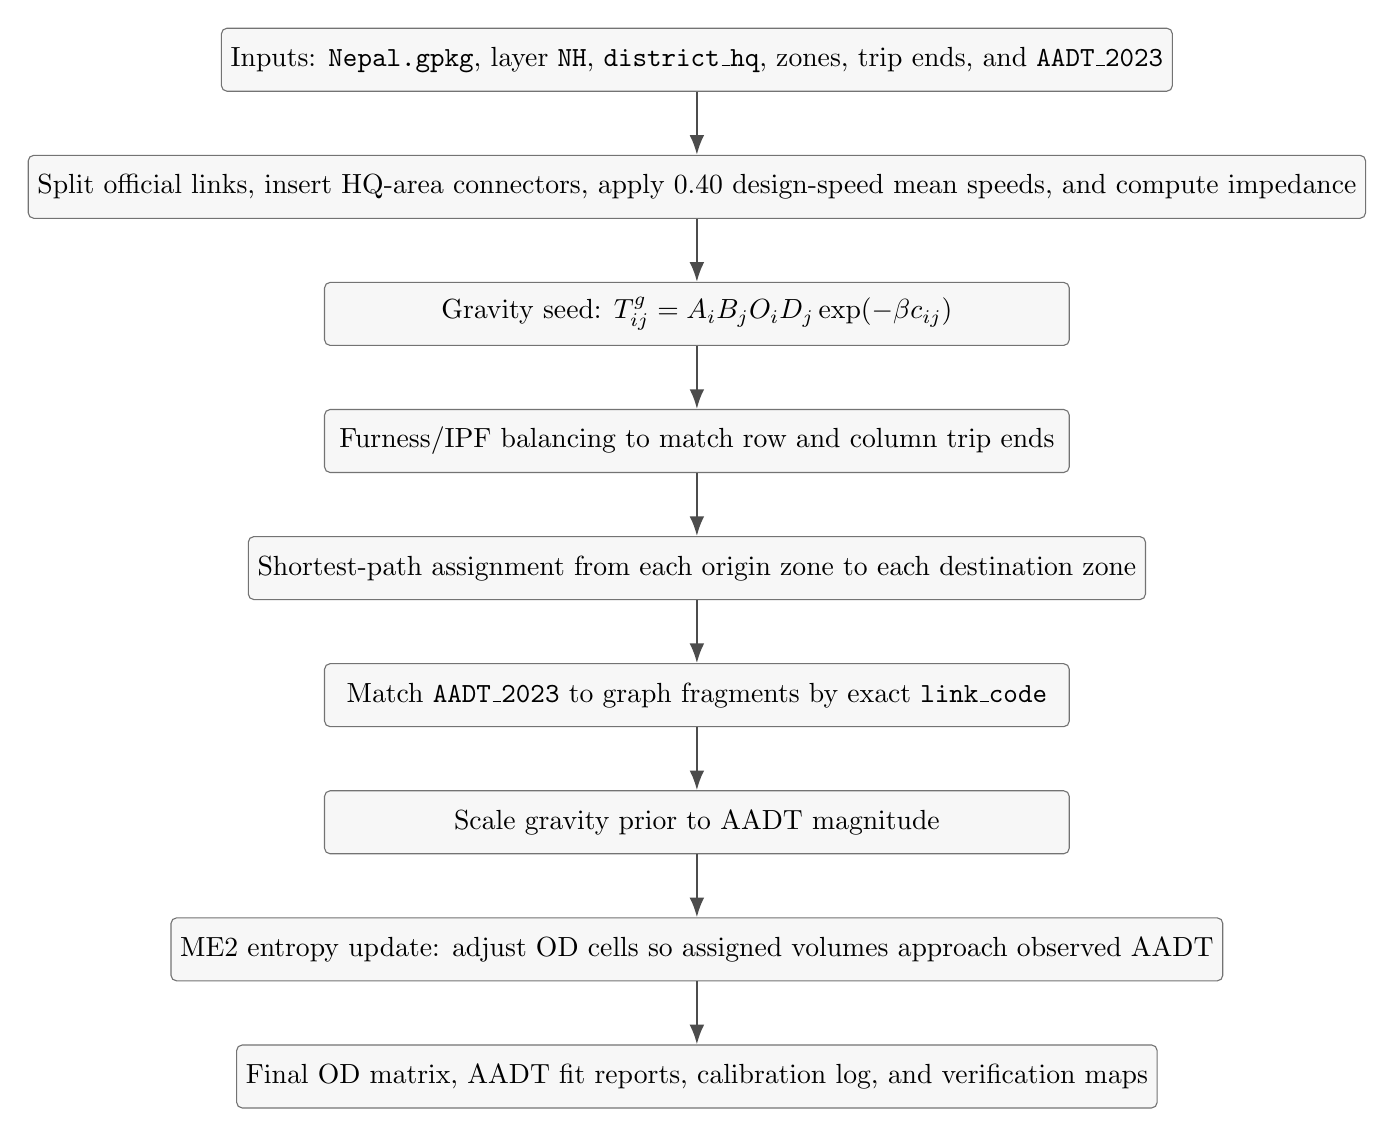
\begin{tikzpicture}[
  node distance=8mm,
  box/.style={rectangle, rounded corners=2pt, draw=black!55, fill=black!3,
              align=center, minimum width=0.78\linewidth, minimum height=8mm},
  arrow/.style={-{Latex[length=2.5mm]}, thick, draw=black!70}
]
\node[box] (input) {Inputs: \texttt{Nepal.gpkg}, layer \texttt{NH}, \texttt{district\_hq}, zones, trip ends, and \texttt{AADT\_2023}};
\node[box, below=of input] (graph) {Split official links, insert HQ-area connectors, apply 0.40 design-speed mean speeds, and compute impedance};
\node[box, below=of graph] (seed) {Gravity seed: $T^{g}_{ij}=A_iB_jO_iD_j\exp(-\beta c_{ij})$};
\node[box, below=of seed] (ipf) {Furness/IPF balancing to match row and column trip ends};
\node[box, below=of ipf] (paths) {Shortest-path assignment from each origin zone to each destination zone};
\node[box, below=of paths] (targets) {Match \texttt{AADT\_2023} to graph fragments by exact \texttt{link\_code}};
\node[box, below=of targets] (scale) {Scale gravity prior to AADT magnitude};
\node[box, below=of scale] (me2) {ME2 entropy update: adjust OD cells so assigned volumes approach observed AADT};
\node[box, below=of me2] (outputs) {Final OD matrix, AADT fit reports, calibration log, and verification maps};
\draw[arrow] (input) -- (graph);
\draw[arrow] (graph) -- (seed);
\draw[arrow] (seed) -- (ipf);
\draw[arrow] (ipf) -- (paths);
\draw[arrow] (paths) -- (targets);
\draw[arrow] (targets) -- (scale);
\draw[arrow] (scale) -- (me2);
\draw[arrow] (me2) -- (outputs);
\end{tikzpicture}
\caption{Implemented OD synthesis and calibration workflow.}
\label{fig:flow}
\end{figure}

\section{Gravity Seed Matrix}

Let $O_i$ be productions from origin zone $i$, $D_j$ be attractions to
destination zone $j$, and $c_{ij}$ be the inter-zonal impedance. The seed matrix
is generated by a doubly constrained gravity model:

\begin{equation}
T^{g}_{ij}=A_iB_jO_iD_jf(c_{ij}), \qquad i\neq j,
\label{eq:gravity}
\end{equation}

with

\begin{equation}
f(c_{ij})=\exp(-\beta c_{ij}).
\label{eq:friction}
\end{equation}

The current run uses $\beta=0.02$. This value is used as an assumed deterrence
parameter for the seed matrix. It is not calibrated from AADT in the present
workflow. Calibrating $\beta$ properly would require observed trip-length
distributions, observed OD information, or a separate gravity-model calibration
dataset. The AADT data enter later as link/section-count evidence.

The balancing factors $A_i$ and $B_j$ are solved iteratively so that the seed
matrix respects the production and attraction totals:

\begin{equation}
\sum_j T^{g}_{ij}=O_i, \qquad \sum_i T^{g}_{ij}=D_j.
\label{eq:constraints}
\end{equation}

The implementation uses Furness/IPF balancing. At each iteration, rows are
scaled to match productions and columns are scaled to match attractions:

\begin{align}
T_{ij} &\leftarrow T_{ij}\frac{O_i}{\sum_j T_{ij}}, \\
T_{ij} &\leftarrow T_{ij}\frac{D_j}{\sum_i T_{ij}}.
\end{align}

This procedure is consistent with the classical Furness method
\cite{furness1965} and with entropy-based trip distribution formulations
\cite{wilson1967,morphet1975}. The diagonal cells are set to zero because this
matrix represents inter-district traffic assignment rather than intra-zonal
movements.

\section{Assignment Representation}

For each non-zero seed OD pair, the script computes the shortest path on the
analysis graph using the travel-time edge weight. This gives the incidence
matrix $P$:

\begin{equation}
p_{ar}=
\begin{cases}
1, & \text{if OD path } r \text{ uses count target } a,\\
0, & \text{otherwise.}
\end{cases}
\label{eq:incidence}
\end{equation}

Here $r$ indexes an OD pair and $a$ indexes an AADT calibration target. The
modelled count at target $a$ is

\begin{equation}
\hat{y}_a = \sum_r p_{ar}x_r = (Px)_a,
\label{eq:count_equation}
\end{equation}

where $x_r$ is the OD demand for pair $r$. This is the core bridge between the
matrix and the AADT observations.

\section{AADT Target Construction}

The first concern in this step was to avoid a misleading calibration. AADT
coverage is incomplete, and the count table does not provide direction. Missing
counts were therefore not interpreted as zero-flow observations. Only observed
AADT rows were allowed to constrain the matrix.

The current run uses the master \texttt{Nepal.gpkg} \texttt{NH} layer directly. A row
is eligible for calibration only if

\begin{equation}
\texttt{AADT\_2023}_i>0 .
\end{equation}

The model uses \texttt{AADT\_2023} as the count target and does not use the
2024/25 field in this pass. The field is deliberately configurable: adding or
editing \texttt{GravityParams} rows such as \texttt{aadt\_value\_field},
\texttt{future\_aadt\_field}, \texttt{master\_gpkg}, and \texttt{road\_layer}
switches the OD calibration source without changing the algorithm. Since all
retained rows come from the selected traffic field, their evidential weight is

\begin{equation}
w_i=1 .
\end{equation}

Because \texttt{link\_code} is preserved from each official highway feature
onto every derived graph fragment, no spatial buffer or route-reference proxy
is needed. For a selected \texttt{AADT\_2023} source link $a$, its selector is
the set $E_a$ of all directed graph fragments with the same unique code.
Incidence is

\begin{equation}
p_{ar}=1 \quad \text{if} \quad E_a\cap E_r\neq\emptyset ,
\end{equation}

where $E_r$ is the edge set of OD path $r$. Both graph directions are included,
so the resulting target is a two-way section count.

For MLPI sensitivity testing, \texttt{Input.xlsx} can optionally supply
supplemental AADT gap-fill values through the
\texttt{Allow Input AADT gap fill} workbook switch.

\begin{table}[H]
\centering
\caption{\texttt{AADT\_2023} target mapping diagnostics.}
\begin{tabular}{lr}
\toprule
\textbf{Mapping diagnostic} & \textbf{Count} \\
\midrule
Positive \texttt{Nepal.gpkg} \texttt{AADT\_2023} rows loaded & 718 \\
Rows matched exactly to graph fragments & Run output \\
Rows unmatched to the current graph & Run output \\
Matched targets before OD-path filtering & Run output \\
Targets crossed by at least one OD shortest path & Run output \\
Targets unused by OD shortest paths & Run output \\
Minimum / median / maximum AADT & 15 / 921 / 58,797 \\
\bottomrule
\end{tabular}
\end{table}

Because the AADT rows are non-directional, the current calibration treats them
as two-way section/screenline information. Directional calibration would require
directional AADT or explicit directed graph-edge IDs.

\section{ME2 / Entropy Calibration}

The seed matrix is treated as a prior matrix $x^0$. In the exact-count form of
the ME2 problem, the matrix is updated by minimising its information distance
from the prior while satisfying the observed counts:

\begin{equation}
\min_{x\geq0}
\sum_r
\left[
x_r\ln\left(\frac{x_r}{x^0_r}\right)-x_r+x^0_r
\right],
\qquad \text{subject to } Px=y.
\label{eq:entropy_objective}
\end{equation}

This information-minimising form is the same family of ideas used by Van
Zuylen and Willumsen \cite{vanzuylen1980}; related maximum-likelihood matrix
estimation formulations are given by Spiess \cite{spiess1987}. More general
work on estimating OD tables from partial link counts is discussed by Sherali
et al. \cite{sherali2003} and Cascetta \cite{cascetta1984}.

The Lagrange multiplier form of the exact entropy solution is

\begin{equation}
x_r=x^0_r\exp\left(\sum_a p_{ar}\lambda_a\right).
\label{eq:me2_solution}
\end{equation}

In the implemented version, counts are incomplete and noisy, so the update is
regularised and damped rather than forced to satisfy every count exactly. The
gravity prior is first globally scaled to the magnitude of the observed AADT:

\begin{equation}
s=\frac{\sum_a w_a y_a}{\sum_a w_a(Px^g)_a},
\qquad x^0=sx^g,
\label{eq:scale}
\end{equation}

where $x^g$ is the raw gravity matrix, $y_a$ is observed AADT, and $w_a$ is the
target weight. With the \texttt{Nepal.gpkg} graph, the numerical
scale factor should be taken from the run-specific \texttt{calibration\_log.csv}.

The multipliers are then updated using the log-ratio between observed and
modelled counts:

\begin{equation}
\lambda^{(k+1)}_a =
(1-\eta\rho)\lambda^{(k)}_a
+\eta\omega
\ln\left(\frac{y_a}{\hat{y}^{(k)}_a}\right),
\label{eq:lambda_update}
\end{equation}

with damping $\eta=0.2$, count weight $\omega=1.0$, and shrinkage $\rho=0.05$.
The OD vector is updated as

\begin{equation}
x^{(k+1)} =
x^0 \circ
\exp\left(P^\top W\lambda^{(k+1)}\right),
\label{eq:implemented_update}
\end{equation}

where $W$ contains the target weights and $\circ$ denotes element-wise
multiplication. The update is clipped to avoid unstable changes from sparse or
locally inconsistent count evidence.

\subsection{What Was Calibrated}

The calibrated object is the OD matrix $x$, not the gravity parameters. In
particular, $\beta$ remains fixed at the value used to create the seed matrix.
This is defensible because AADT is link-count information, not a direct
trip-length distribution or observed OD sample. It can tell us that assigned
traffic on a section is too high or too low, but it does not uniquely identify
the gravity impedance parameter without additional assumptions.

The final OD values are therefore best described as:

\begin{quote}
Daily inter-district OD trips in units consistent with the selected AADT
evidence after entropy-based updating of a gravity prior.
\end{quote}

\section{Calibration Diagnostics}

\begin{table}[H]
\centering
\caption{Pre-ME2 diagnostics reported by the current Nepal.gpkg configuration.}
\begin{tabular}{lr}
\toprule
\textbf{Diagnostic} & \textbf{Value} \\
\midrule
OD paths found & Run output \\
Active 2023 AADT targets after path filtering & Run output \\
Raw gravity seed total trips & Run output \\
Global AADT scale factor before ME2 & Run output \\
Scaled gravity seed total trips & Run output \\
Raw seed RMSE against active 2023 targets & Run output \\
Scaled seed RMSE against active 2023 targets & Run output \\
\bottomrule
\end{tabular}
\end{table}

The full final OD values, convergence statistics and largest OD table are
reported from the run outputs. The current OD calibration uses
\texttt{AADT\_2023} as its traffic-count evidence.

\section{Map-Based Verification}

Two verification maps were generated to make the calibration auditable:

\begin{enumerate}
    \item an AADT map showing \texttt{AADT\_2023} sections from
    \texttt{Nepal.gpkg}, labelled by link code and AADT; and
    \item a major-OD map showing the largest final OD cells along the same
    shortest paths used to construct the ME2 path-incidence matrix.
\end{enumerate}

Each figure contains a national overview and separate western, central, and
eastern panels. Detailed panels use small collision-filtered labels. The map
geometry is simplified only for display; matching, assignment, calibration,
and reported values use the original network geometry.

The routed OD map does not use straight desire lines or a separate illustrative
road layer. For each displayed OD cell, the saved edge sequence in
\texttt{od\_pair\_path\_features.csv} is joined back to
\texttt{GraphEdges.gpkg}. This graph was derived from
\texttt{Nepal.gpkg} and is the same network representation used to
calculate the impedance matrix. Thus, the displayed line is the modelled road
route associated with that OD cell. It should still be described as an
estimated routed OD movement, rather than an independently observed ``actual''
OD trip.

\begin{figure}[H]
\centering
\figurepanel{figures/aadt_nh_2023_overview_regions.pdf}{AADT\_2023 on Nepal.gpkg highway sections.}
\caption{Two-way AADT from \texttt{Nepal.gpkg}, layer \texttt{NH}, field
\texttt{AADT\_2023}.
This figure is produced by the verification-map workflow.}
\label{fig:aadtmap}
\end{figure}

\begin{figure}[H]
\centering
\figurepanel{figures/major_od_routed_paths_overview_regions.pdf}{Top final OD movements on modelled shortest paths.}
\caption{Largest directed OD cells from the calibrated matrix plotted along
their modelled shortest paths. A label is an OD-matrix value, not an aggregate
link volume. Shared road sections may therefore carry several labelled OD
movements.}
\label{fig:odmap}
\end{figure}

\section{Outputs}

\begin{table}[H]
\centering
\caption{Default output files from the current OD run.}
\begin{tabularx}{\linewidth}{p{0.36\linewidth} X}
\toprule
\textbf{Output} & \textbf{Meaning} \\
\midrule
\texttt{od\_matrix\_ids.csv} &
Final 77 $\times$ 77 calibrated OD matrix using zone IDs. \\
\texttt{od\_matrix\_names.csv} &
Final OD matrix with district/HQ labels for MLPI and manual inspection. \\
\texttt{optional diagnostics} &
Seed matrices, OD-pair tables, path-incidence features, AADT mapping reports,
fit reports, calibration logs and verification-map inputs are opt-in
diagnostics controlled by \texttt{GravityParams} switches such as
\texttt{write\_diagnostics}, \texttt{write\_seed\_outputs},
\texttt{write\_pair\_table}, and \texttt{write\_summary}. \\
\bottomrule
\end{tabularx}
\end{table}

\section{Interpretation and Limitations}

The current matrix is useful because it combines three pieces of information:
district-level trip-end structure, network impedance, and observed traffic
counts. The strongest part of the method is that AADT observations are retained
as observations only where they exist. Unobserved links remain unconstrained.

The main limitations are:

\begin{itemize}
    \item The 2023 AADT field is non-directional, so calibration remains two-way
    section/screenline calibration even though link-code matching is exact.
    \item Any unmatched or unused 2023 AADT targets should be reported from the
    run-specific \texttt{aadt\_mapping\_report.csv} and
    \texttt{assignment\_targets.csv}.
    \item The impedance uses 40\% of source design speed as average operating
    speed. It still does not explicitly represent congestion, pavement
    condition, weather or seasonal closure.
    \item District-HQ connectors now use the \texttt{Nepal.gpkg}
    \texttt{district\_hq} area geometry directly. A large connector distance is
    a network-access QA item, not evidence that the HQ was a disconnected point.
    \item The ME2 update does not preserve gravity-model trip ends in the
    current configuration. This lets counts influence total demand, but it also
    means final row/column totals can differ from the seed totals.
    \item The gravity deterrence parameter was assumed, not estimated from
    observed trip-length data.
\end{itemize}

For a stronger next version, the most valuable additions would be directional
AADT splits, observed operating speeds and explicit local-road access
connectors beyond the national-highway graph.

\section{Conclusion}

The final OD matrix should be described as a calibrated daily inter-district
demand matrix in the same units as the selected AADT evidence. With the current
configuration, that evidence is \texttt{AADT\_2023} from
\texttt{Nepal.gpkg}. Methodologically, the estimate is not just a gravity
matrix and it is not a forced copy of AADT values. It is a gravity prior
updated through an entropy-based count-calibration step. The revised
implementation keeps the impedance graph tied to \texttt{Nepal.gpkg}, uses
the \texttt{district\_hq} area layer for closest-point HQ connectors, applies
the \texttt{NH} design-speed field with a 0.40 mean-speed factor for
travel-time impedance, and constructs AADT selectors from exact
\texttt{Nepal.gpkg} \texttt{NH} link codes.

\begin{thebibliography}{99}

\bibitem{banjara2023}
Banjara, B. P., and Gautam, G. (2023).
\newblock A case study on the effect of geometric design consistency on road
crashes on Narayanghat--Muglin road section.
\newblock \emph{SCITECH Nepal}, 17(1), 58--63.
\newblock \url{https://doi.org/10.3126/scitech.v17i1.60469}.

\bibitem{bist2024}
Bist, T. C., and Tiwari, H. (2024).
\newblock Assessment of stratified speed characteristics and compliance with
posted speed limit in an urban area: A case study of section of Karnali
Highway, Nepal.
\newblock \emph{International Journal on Engineering Technology}, 2(1),
187--194.
\newblock \url{https://doi.org/10.3126/injet.v2i1.72571}.

\bibitem{dor2013}
Department of Roads. (2013).
\newblock \emph{Nepal Road Standard 2070}.
\newblock Government of Nepal.

\bibitem{dor2023}
Department of Roads. (2023).
\newblock \emph{Main report of detailed design of upgradation of
Butwal--Gorusinghe Road}.
\newblock Ministry of Physical Infrastructure and Transport, Government of
Nepal.
\newblock \url{https://dor.gov.np/dorfcb/publication/access-mpa-phase-1/main-report-of-butwal-gorusinghe-road}.

\bibitem{jica2022}
Japan International Cooperation Agency and Department of Roads. (2022).
\newblock \emph{The project on improvement of Kathmandu Ring Road (Phase II):
Preparatory survey final report}.
\newblock Japan International Cooperation Agency.
\newblock \url{https://openjicareport.jica.go.jp/pdf/12382388_01.pdf}.

\bibitem{ktmtraffic2023}
Kathmandu Valley Traffic Police Office. (2023).
\newblock Notice on speed limits for major roads in Kathmandu Valley.
\newblock Reported in OnlineKhabar English.
\newblock \url{https://english.onlinekhabar.com/50-kmph-speed-limit-kathmandu.html}.

\bibitem{joshi2022}
Joshi, E., Gautam, P., Khadka, A., Pilkington, P., Parkin, J., Joshi, S. K.,
and Mytton, J. (2022).
\newblock Experience of living near a highway in Nepal: Community perceptions
of road dangers in Makwanpur district.
\newblock \emph{Journal of Transport \& Health}, 24, 101337.
\newblock \url{https://doi.org/10.1016/j.jth.2022.101337}.

\bibitem{wilson1967}
Wilson, A. G. (1967).
\newblock A statistical theory of spatial distribution models.
\newblock \emph{Transportation Research}, 1, 253--269.
\newblock \url{https://doi.org/10.1016/0041-1647(67)90035-4}.

\bibitem{furness1965}
Furness, K. P. (1965).
\newblock Time function iteration.
\newblock \emph{Traffic Engineering and Control}, 7(7), 458--460.

\bibitem{morphet1975}
Morphet, R. (1975).
\newblock A note on the calculation and calibration of doubly constrained trip
distribution models.
\newblock \emph{Transportation}, 4, 43--53.
\newblock \url{https://doi.org/10.1007/BF00166888}.

\bibitem{evans1973}
Evans, S. P. (1973).
\newblock A relationship between the gravity model for trip distribution and
the transportation problem in linear programming.
\newblock \emph{Transportation Research}, 7(1), 39--61.
\newblock \url{https://doi.org/10.1016/0041-1647(73)90005-1}.

\bibitem{vanzuylen1980}
Van Zuylen, H. J. and Willumsen, L. G. (1980).
\newblock The most likely trip matrix estimated from traffic counts.
\newblock \emph{Transportation Research Part B: Methodological}, 14(3),
281--293.
\newblock \url{https://doi.org/10.1016/0191-2615(80)90008-9}.

\bibitem{cascetta1984}
Cascetta, E. (1984).
\newblock Estimation of trip matrices from traffic counts and survey data: A
generalized least squares estimator.
\newblock \emph{Transportation Research Part B: Methodological}, 18(4--5),
289--299.
\newblock \url{https://doi.org/10.1016/0191-2615(84)90012-2}.

\bibitem{spiess1987}
Spiess, H. (1987).
\newblock A maximum likelihood model for estimating origin-destination
matrices.
\newblock \emph{Transportation Research Part B: Methodological}, 21(5),
395--412.
\newblock \url{https://doi.org/10.1016/0191-2615(87)90037-3}.

\bibitem{sherali2003}
Sherali, H. D., Narayanan, A., and Sivanandan, R. (2003).
\newblock Estimation of origin-destination trip-tables based on a partial set
of traffic link volumes.
\newblock \emph{Transportation Research Part B: Methodological}, 37(9),
815--836.
\newblock \url{https://doi.org/10.1016/S0191-2615(02)00073-5}.

\end{thebibliography}

\end{document}
